\documentclass{article}
\usepackage{v-test-paper}

%\renewcommand{\ans}{\textcolor{red!95}{\textit{\quad}}}
%\def\ansit#1{\textcolor{red!95}{\quad}}

\title{Module-Test-9\\(Physics-JEE)}

% 01. Friction
% 02. Impulse
% 03. Rocket propulsion
% 04. Work Done


\begin{document}
\maketitle

\jeeSectionA

\begin{enumerate}
\item A ball of mass $m$ moving with velocity $v_0$ collides a wall as shown in figure. After impact it rebounds with a velocity $\dfrac{3}{4}v_0$. The impulse acting on ball during impact is
\begin{center}
\begin{tikzpicture}
\tzline+[->](1, 0)(1, 0){$x$}[r]
\tzline+[->](1, 0)(0, -1){$y$}[b]
\pic[rotate=90] {frame=4cm};
\tzline+[dashed](0, 0)(-2, 0)
\coordinate  (a) at (-2, 1.5);
\coordinate  (b) at (-2, -2.6);
\tzdot*(a)(10pt)
\tzdot*(b)(10pt)
\tzline[-->--](a)(0, 0)
\tzline[-->--](0, 0)(b)
\tzanglemark(a)(0, 0)(-2, 0){$37^\circ$}(15pt)
\tzanglemark(-2, 0)(0, 0)(b){$53^\circ$}(18pt)
\end{tikzpicture}
\end{center}
\begin{tasks}(2)
	\task $-\dfrac{1}{2}mv_0\hat{j}$
	\task $-\dfrac{3}{4}mv_0\hat{i}$
	\task $-\dfrac{5}{4}mv_0\hat{i}$\ans
	\task None of these
\end{tasks}

\item A bucket tied to a string is lowered at a constant acceleration of $g/4$. If mass of the bucket is $m$ and it is lowered by a distance $l$ then find the work done by the string on the bucket.
\begin{tasks}(2)
	\task $-\dfrac{3}{4}mgl$\ans
	\task $\dfrac{3}{4}mgl$
	\task $\dfrac{4}{3}mgl$
	\task $-\dfrac{4}{3}mgl$
\end{tasks}

\item A block is constrained to move along x-axis under a force $F = - 2x$ . Here, $F$ is in newton and $x$ in
metre. Find the work done by this force when the block is displaced from $x = 2 \m$ to $x = - 4 \m$.
\begin{center}
\begin{tikzpicture}
\pic {frame=5cm};
\node[block] at (-1, 0.4)(block){};
\tzline+[->](block.east)(1.5, 0){$F$}[r]
\end{tikzpicture}
\end{center}
\begin{tasks}(2)
	\task $12\Joule$
	\task $-12\Joule$\ans
	\task $8\Joule$
	\task $-8\Joule$
\end{tasks}

\item Displacement of a particle of mass $2 \kg$ varies with time as $s = (2t^2 - 2t + 10) \m$. Find total work done on the particle in a time interval from $t = 0$ to $t = 2 \s$.
\begin{tasks}(2)
	\task $-32\Joule$
	\task $16\Joule$
	\task zero
	\task $32\Joule$\ans
\end{tasks}

\item A $5\kg$ mass is raised a distance of $4\m$ by a vertical force of $80\N$. Find the final kinetic energy of the mass if it was originally at rest. $g = 10\mpss$.
\begin{tasks}(2)
	\task $100\Joule$
	\task $-100\Joule$
	\task $120\Joule$\ans
	\task None of these
\end{tasks}

\item Work done when a force $F=(\hat{i}+2\hat{j}+3\hat{k})\N$ acting on a particle takes it from the point $\vec{r}_1 = (\hat{i} + \hat{j} + \hat{k} )$ to the point $\vec{r}_2 = (\hat{i} - \hat{j} + 2 \hat{k} )$ is
\begin{tasks}(2)
	\task $-3\Joule$
	\task $-1\Joule$\ans
	\task zero
	\task $2\Joule$
\end{tasks}

\item When a rubber band is stretched by a distance $x$ , it
exerts a restoring force of magnitude $F = ax + bx^2$, where, $a$ and $b$ are constants. The work done in stretching the unstretched rubber band by $L$ is
\begin{tasks}(2)
	\task $aL^2+bL^3$
	\task $\dfrac{1}{2}\left(aL^2+bL^3\right)$
	\task $\dfrac{aL^2}{2} + \dfrac{bL^3}{3}$\ans
	\task $\dfrac{1}{2}\left( \dfrac{aL^2}{2} + \dfrac{bL^3}{3} \right)$
\end{tasks}



\item The minimum stopping distance of a car moving with velocity $v$ is $x$. If the car is moving with velocity $2v$, then the minimum stopping distance will be
\begin{tasks}(2)
	\task $2x$
	\task $4x$\ans
	\task $3x$
	\task $8x$
\end{tasks}

\item A spring of force constant $k$ is cut in two parts at its one-third length. When both the parts are stretched by same amount. The work done in the two parts will be
\begin{tasks}(2)
	\task equal in both
	\task greater for the longer part
	\task greater for the shorter part\ans
	\task data insufficient
\end{tasks}

\item A force $F=(3t\hat{i}+5\hat{j})\N$ acts on a body due to which its displacement varies as $S=(2t^2\hat{i}-5\hat{j})\m$. Work done by this force in $2\s$ is
\begin{tasks}(2)
	\task $32\Joule$
	\task $24\Joule$\ans
	\task $46\Joule$
	\task $20\Joule$
\end{tasks}

\item Under the action of a force, a $2 \kg$ body moves such that its position $x$ as a function of time is given by $x=\dfrac{t^3}{3}$, where $x$ is in metre and $t$ in second. The work done by the force in the first two seconds is
\begin{tasks}(2)
	\task $1600\Joule$
	\task $160\Joule$
	\task $16\Joule$\ans
	\task $1.6\Joule$
\end{tasks}

\item A bomb of mass $9 \kg$ explodes into two pieces of masses $3 \kg$ and $6 \kg$. The velocity of mass $3 \kg$ is $16\mps$. The kinetic energy of mass $6 \kg$ is
\begin{center}
\begin{tikzpicture}
\tzdot*(0, 0)(25pt)
\tzdot*(3, 1)(15pt)
\tzdot*(3, -1)(12pt)
\tzline+[->](3, 1)(1, 1){$v$}[ar]
\tzline+[->](3, -1)(1, -1){$16\mps$}[br]
\end{tikzpicture}
\end{center}
\begin{tasks}(2)
	\task $96\Joule$
	\task $384\Joule$
	\task $192\Joule$\ans
	\task $768\Joule$
\end{tasks}


\item A rocket of mass $m_0$ has attained a speed equal to its exhaust speed and at that time the mass of
the rocket is $m$. Then the ratio $\dfrac{m_0}{m}$ is ( neglect gravity )
\begin{tasks}(2)
	\task $2.718$\ans
	\task $7.8$
	\task $3.14$
	\task $4$
\end{tasks}

\item A jet of water hits a flat stationary plate perpendicular to its motion. The jet ejects $500\gm$ of water per second with a speed of $1 \mps$. Assuming that after striking, the water flows parallel to the plate, then the force exerted on the plate is
\begin{tasks}(2)
	\task $5\N$
	\task $1\N$
	\task $0.5\N$\ans
	\task $10\N$
\end{tasks}

\item A rocket of mass $40 \kg$ has $160 \kg$ fuel. The exhaust velocity of the fuel is $2.0 \kmps$. The rate of consumption of fuel is $4 \kg/\s$. Calculate the ultimate vertical speed gained by the rocket. ($g = 10 \mpss$)
\begin{tasks}(2)
	\task $1.82\kmps$
	\task $2.82\kmps$\ans
	\task $3.82\kmps$
	\task $4.82\kmps$
\end{tasks}

\item A ball of mass $1 \kg$ is attached to an inextensible string. The ball is released from the position shown in figure. Find the impulse imparted by the string to the ball immediately after the string becomes taut. (Take $g = 10 \mpss$)
\begin{center}
\begin{tikzpicture}
\pic[rotate=180] {frame=2cm};
\tzline+(0, 0)(0, -2)
\tzarc(0.25, -2)(180:360:0.25)
\tzline+(0.5, -2)(0, 1)
\tzdot*(0.5, -1)(10pt)
\tzline[|<->|](1, -2.25)(1, -1){$1\m$}[midway, right]
\end{tikzpicture}
\end{center}
\begin{tasks}(2)
	\task $2\sqrt{10}\N\s$\ans
	\task $3\sqrt{10}\N\s$
	\task $4\sqrt{10}\N\s$
	\task $5\sqrt{10}\N\s$
\end{tasks}

\item Velocity-time graph of a particle of mass $2 \kg$ moving in a straight line is as shown in figure shown. Find the work done by all the forces acting on the particle.
\begin{center}
\begin{tikzpicture}
\tzaxes(-0.5, -0.5)(4, 3){$t(\s)$}{$v(\mps)$}
\tzline(0, 2.5)(3, 0)
\tzticks{3/$2$}{2.5/$20$}
\end{tikzpicture}
\end{center}
\begin{tasks}(2)
	\task $400\Joule$
	\task $-400\Joule$\ans
	\task $20\Joule$
	\task $-20\Joule$
\end{tasks}

\item If a ladder weighing $250 \N$ is placed against a smooth vertical wall having coefficient of friction between it and floor $0.3$, then what is the maximum force of friction available at the point of contact between the ladder and the floor?
\begin{tasks}(2)
	\task $75\N$
	\task $50\N$
	\task $35\N$
	\task $25\N$\ans
\end{tasks}

\item A block of mass $4 \kg$ is placed on a rough horizontal plane. A time dependent horizontal force $F = kt$ acts on the block. Here $k = 2 \N/\s$. The frictional force between the block and plane at
time $t = 2\s$ is ($\mu = 0.2$)
\begin{tasks}(2)
	\task $4\N$
	\task $8\N$\ans
	\task $12\N$
	\task $10\N$
\end{tasks}

\item A force $F_1$ accelerates a particle from rest to a velocity $v$. Another force $F_2$ decelerates the same particle from $v$ to rest, then
\begin{tasks}(1)
	\task $F_1$ is always equal to $F_2$\ans
	\task $F_2$ is greater than $F_1$
	\task $F_2$ may be smaller than, greater than or equal to $F_1$
	\task $F_2$ cannot be equal to $F_1$
\end{tasks}

\end{enumerate}



\jeeSectionB


\begin{enumerate}
\item Momentum of a particle is increased by 50\%. By how much percentage kinetic energy of particle
will increase ?
\ansit{125}

\item Kinetic energy of a particle is increased by 2\%. By how much percentage momentum of the particle will increase ? \ansit{1}

\item The average resisting force that must act on a $5 \kg$ mass to reduce its speed from $65\mps$ to $15 \mps$ in $2\s$ is \ansit{125}

\item A time dependent force $F = 6t$ acts on a particle of mass $1 \kg$. If the particle starts from rest, the work done by the force during the first $1 \s$ will be $k.5\Joule$, then the value of $k$ is \ansit{4}

\item A block of mass $0.5 \kg$ has an initial velocity of $10 \mps$ while moving down an inclined plane of angle $30^\circ$, the coefficient of friction between the block and the inclined surface is $0.2$. The velocity of the block, after it covers a distance of $10 \m$, is \ansit{13}

\item A particle moves along the x-axis from $x = 0$ to $x = 5 \m$ under the influence of a force given by $F = 7 - 2 x + 3 x^2$. The work done(in Joule) in the process is\ansit{135}


\item A block of mass $5\kg$ is lifted slowly against the gravity for $5\m$ then the work done(in Joule) by the external force which is responsible for the lifting of the block is \ansit{250}

\item A force of $(5+3x) \N$ acting on a body of mass $20 \kg$ along the x-axis displaces it from $x=2\m$ to $x=6\m$. The work done(in Joule) by the force is \ansit{68}

\item Suppose you punched your fist into a solid-wall perpendicularly with a speed of $5\mps$, then what would be the impulse you will feel if the mass of your hand is $2\kg$ ?\ansit{10}

\item If a particle is moving in a conservative force field, then what would be the be work done by this field in moving this particle from $x=5$ to $x=10$ then back to $x=5$ ?\ansit{0}


	
\end{enumerate}


\end{document}
